\documentclass[12pt]{article}
\usepackage[margin=1in]{geometry} 
\usepackage{amsmath,amsthm,amssymb,amsfonts}
\usepackage{dirtytalk}
\usepackage{flexisym}
\usepackage{tikz}
\usepackage{tikz-cd}
\usepackage{listings}
\usepackage{graphicx}
\usepackage{caption}
\usepackage{subcaption}
\usepackage{multicol}
\usepackage{algorithm}
\usepackage{array}
\usepackage[noend]{algpseudocode}
 
\newcommand{\N}{\mathbb{N}}
\newcommand{\Z}{\mathbb{Z}}
 
\newenvironment{problem}[2][Problem]{\begin{trivlist}
\item[\hskip \labelsep {\bfseries #1}\hskip \labelsep {\bfseries #2.}]}{\end{trivlist}}
%If you want to title your bold things something different just make another thing exactly like this but replace "problem" with the name of the thing you want, like theorem or lemma or whatever
 
\begin{document}
 
%\renewcommand{\qedsymbol}{\filledbox}
%Good resources for looking up how to do stuff:
%Binary operators: http://www.access2science.com/latex/Binary.html
%General help: http://en.wikibooks.org/wiki/LaTeX/Mathematics
%Or just google stuff
 
\title{Math 410 Report}
\author{Jonathan Pearce, 260672004}
\maketitle

\section{Introduction}
Over the past decade, the rate of drug attrition due to clinical trial failures has risen substantially. Unfortunately it is difficult to identify compounds that have unfavourable toxicity properties before conducting clinical trials. In 2016 Researchers from Cornell University developed a new data-driven approach (PrOCTOR) [1], that directly predicts the likelihood of toxicity in clinical trials using the random forest learning algorithm. Using the properties of a compounds targets and its structure as input, PrOCTOR is able to predict whether the drug will fail clinical trials due to toxicity. In this project I investigated the potential of modifying PrOCTOR's prediction capabilities to be driven by gradient boosting instead of random forest. Previously, gradient boosting has been found to be more successful at prediction in general than random forest [2,3]. During this project we conducted testing with gradient boosting models, both with the full feature set from our data as well as a reduced feature set. Further our own original testing with a random forest model was completed to aid in comparison between the two types of learning algorithms. Our gradient boosting version of PrOCTOR proved to be very effective and slightly outperformed the results of PrOCTOR in the selected evaluation metric. Follow up analysis' concluded that the entire feature set was critical if one wants optimal performance from the model and further our gradient boosting model outperformed our random forest model on the same data further supporting the idea that gradient boosting is a more powerful tool at predicting drug failures in this setting.

\section{Data Collection}
One of the main goals of this project was to ensure my results with the gradient boosting version of PrOCTOR would be comparable to the results reported for PrOCTOR in the original 2016 paper. Therefore the first step in the project was to acquire a dataset that was comparable to the original data set used to train PrOCTOR with respect to the feature set and number of samples. The researchers who developed PrOCTOR have made the code available on Github [4], however, they do not list any datasets that were used in their training and testing. After looking through all the files on the Github account I found that the Proctor.rds file had a data set saved as a variable, I was able to export and save this dataset through RStudio. This dataset contained 846 drugs and had all 48 features used by PrOCTOR for each drug. The original data used for training PrOCTOR had 884 drugs, therefore it is likely that this data set is a large subset of the original data set, with only 38 drugs removed. Finding a dataset with all of the necessary features was a big assistance throughout this entire project, it made the final results more accurate and comparable to the PrOCTOR results. Further it meant I did not need to replicate there data collection techniques. The only issue with this dataset was that it was unlabelled, there was no distinction between which drugs had failed their clinical trial due to toxicity and which were FDA approved. In order to classify each drug in the dataset I had to parse through the clinical trial database and find an accurate method to give each drug the proper label. \\
The entire clinical trial database can be downloaded online [5]. The format of the database was updated towards the end of 2016 to allow for more easy data access. Since the PrOCTOR paper was published on September 15, 2016, I figured the researchers from Cornell most likely had used the copy of the database from March 2016 (prior to the format update). I downloaded the pipe delimited text files and reformatted the 'clincal_study.txt' file to contain one clinical trial per line of text to make parsing and filtering the file easier. With the newly formatted 'clincal_study.txt' file I followed the same procedure for finding drugs that failed a trial due to toxicity reasons as is outlined in the PrOCTOR paper. I checked each clinical trial for the words 'suspended','terminated' or 'withdrawn' as well as 'toxic', every clinical trial in the text file that met this criteria was written to a new text file that held all trials that could potentially contain a failed drug. Studies that were stopped because of poor accrual were removed from this set of candidates. With this new text file I iterated through the list of 846 drugs in my data set and checked whether any of them were in this text file of candidate failed trials, any drug that was in the file was tagged as a drug that failed due to toxicity reasons. Following this procedure I was left with a list drugs that had failed a clinical trial due to toxicity reasons and was in my dataset, the remaining drugs in the dataset were considered to be from the set of FDA approved drugs. A visual inspection of the newly labelled response variable for each drug saw a large concentration of these drugs grouped at the top of the dataset, about 80\% of these drugs were found in the first 100 drugs in the data set. This made it seem likely that the true drugs that had failed due to toxicity reasons were actually all at the top of the dataset file. I followed up by reviewing the outlier drugs that were not caught by my database parser by hand and realized that many were edge cases that my code would not have caught and they were in fact drugs that failed due toxicity reasons as well. After correcting these discrepancies, there were 86 drugs that had failed a clinical trial due to toxicity reasons in my dataset. I was confident that my data set was complete and accurate and was ready to be used to train and test the gradient boosting version of PrOCTOR.

\section{Analysis}
Throughout the analysis I attempted to follow the process outlined in the PrOCTOR paper as closely as possible so as to make the comparison between methods as accurate as possible. To ensure I fairly compared the two types of learning algorithms I also replicated the PrOCTOR algorithm with my own random forest model to assist with comparisons. This allowed me to compare my gradient boosting prediction technique to both the original PrOCTOR algorithm and my own random forest model. \\
To begin, I mimicked the PrOCTOR paper and did principal component analysis on the 34 target features. These features were highly correlated. As was the case for PrOCTOR I replaced the 34 target features with the first three principle components. PCA helped reduce the dimensionality of our feature space significantly, from 48 total features to 17 features. These principle components were not well correlated with the rest of the features indicating that they add information that was independent of the chemical features and chemical properties of the drugs. This was the only data preprocessing outlined in the paper. \\
The next step was to divide the data into a training set and test set. This proved to be difficult because of the class imbalance in the data; 86 drugs that failed due to toxicity, 760 drugs that are FDA approved. At first I attempted to simply split both sets of classes evenly, and put one half in the training set and one half in the test set for each class. However allowing this large an imbalance in the training set meant that any model trained on this data would simply learn to predict FDA drug for every instance, since there were almost ten times as many samples from the FDA approved class. It was evident this technique would not work and another process needed to be implemented. The next time the training set was given 50 samples from each class leaving a test set with 36 drugs that failed due to toxicity and 710 drugs that were FDA approved. There was still significant imbalance in the test set which meant that the choice of evaluation metric would be critical. The basic accuracy metric does a very poor job accounting for class imbalance so it was not an option in this case. The next metric I considered was area under the curve (AUC), this metric ranges from 0.5 (random guessing) to 1 (a perfect classifier) and can be depicted visually on a 2D graph, where the true positive rate of the classifier (sensitivity) is compared against the false positive rate (1 - specificity). This metric does a good job of ignoring class imbalance and provides an accurate evaluation of model prediction power, therefore it seemed like a good choice for the classifier evaluation metric. Further in the PrOCTOR paper, area under the curve was the metric reported for the original dataset, this makes the comparison between PrOCTOR's and my model's performance straightforward. \\
Following this the gradient boosting model was trained. All 17 features (10 molecular properties, 4 drug-likeness rule features, and 3 principle components of target based properties) were used in the training process, since PrOCTOR was trained on the same 17 features. The gbm R package was used for the gradient boosting algorithm. XGBoost which has gained a lot of popularity recently was also considered, however XGBoost is designed for very large datasets. In training the gradient boosting model I specified the number of trees, interaction depth, shrinkage as well as the number of cross validation folds. Through empirical testing I found effective parameters to be: interaction depth = 6, shrinkage = 0.001, CV_folds = 5. The 'perf' function was utilized to ensure the optimal number of trees were chosen for prediction. The error function for the gradient boosting model is below, and the optimal number of trees was found to be 4402 (Figure 1).
\begin{figure}[h!]
\centering
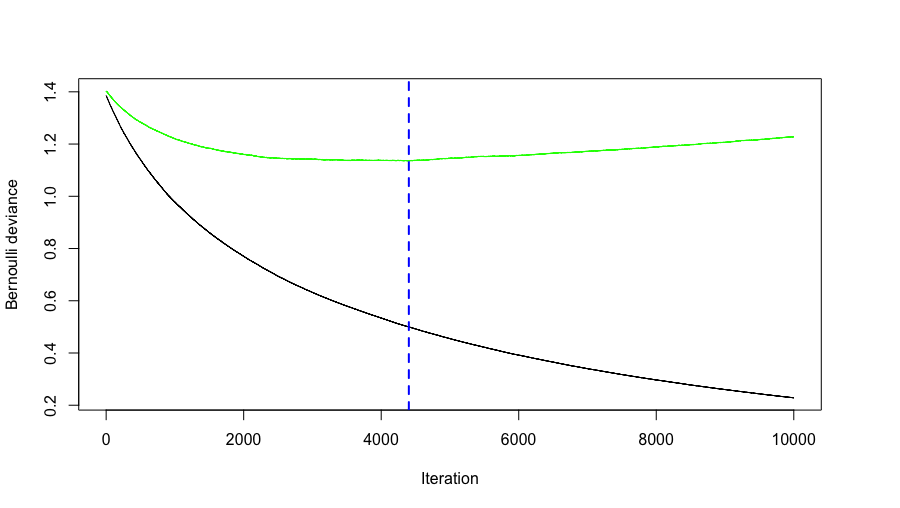
\includegraphics[width=12cm]{GBfullperf.png}
\label{fig:sub1}
  \caption{Error measurement for Gradient Boosting Model}
\end{figure}

Following the parameter tuning and with the optimal number of trees, the gradient boosting model proceeded to classify the 746 drugs in the test set. The gradient boosting version of PrOCTOR had significant predictive performance and achieved an area under the curve score of 0.8312 (Figure 2).
\begin{figure}[h!]
\centering
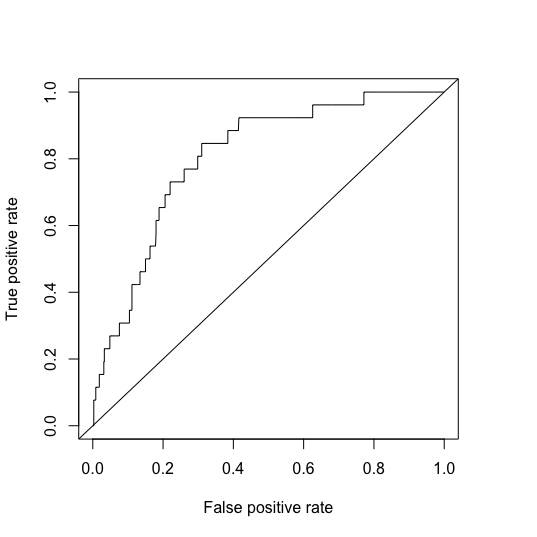
\includegraphics[width=9cm]{GBFullAUC.png}
  \label{fig:sub1}
  \caption{Gradient Boosting Model Performance}
\end{figure}

These strong results demonstrated the predictive power of gradient boosting. The area under the curve score of this new gradient boosting model had surpassed that of the PrOCTOR algorithm with the original dataset (AUC = 0.8263). Following this promising performance, a follow up was conducted with a subset of the 17 model features. The goal was to see whether a reduced feature set could have comparable performance. A smaller yet equally effective feature set would have two advantages, it would speed up model training if the dataset size was ever expanded, further a smaller set of features would be less expensive, in terms of time when collecting data. In the PrOCTOR paper they discuss that, the first expression principle component, QED metric, polar surface area, and the drug target’s network connectivity emerged as the four most important features. This seemed like a logical subset of features to try since it was clear they were effective features and this set of features was significantly smaller than the previous set (13 less features), and would thus actually help with data collection speed in the future. The same process as above was carried out with a gradient boosting model, the optimal number of trees was found to be 6427, and the proceeding prediction process resulted in an area under of the curve score of 0.7862 (Figure 3).

\begin{figure}[h!]
\centering
\begin{subfigure}{.5\textwidth}
  \centering
  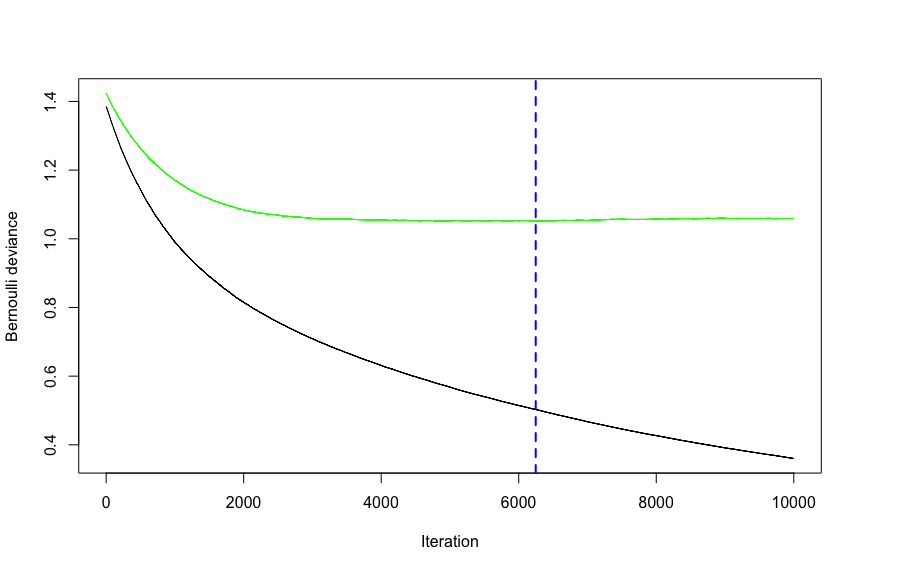
\includegraphics[width=0.95\linewidth]{GBSimpleperf.png}
  \label{fig:sub1}
\end{subfigure}%
\begin{subfigure}{.5\textwidth}
  \centering

  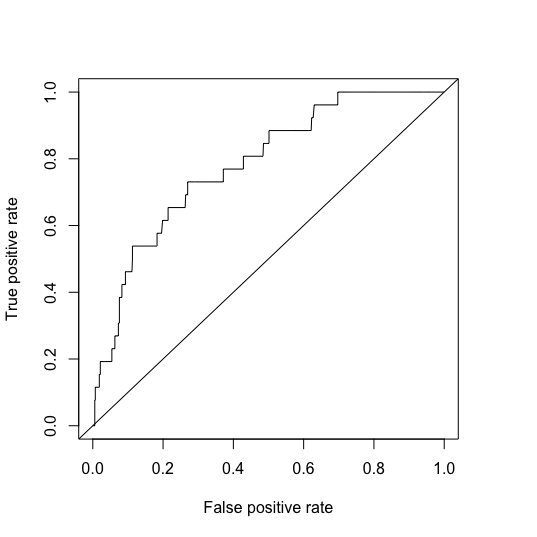
\includegraphics[width=0.95\linewidth]{GBSimpleAUC.png}
  \label{fig:sub2}
\end{subfigure}
\label{fig:test}
\caption{Error measurement and performance of Gradient Boosting Model with reduced feature space}
\end{figure}

The performance of the gradient boosting model with the reduced set of features failed to match the performance of the first gradient boosting model or PrOCTOR's performance. From this it appears that there is significant information in the excluded 13 features that aid in prediction.  \\ 
To help make more significant comparisons between the random forest and gradient boosting learning algorithms with respect to predicting clinical trail failure due to toxicity with this data set, the same procedure was completed to train a random forest model. The random forest model was provided all 17 features and the same training and test set as the gradient boosting models. The model produced an area under the curve score of 0.803 (Figure 4).

\begin{figure}[h!]
\centering
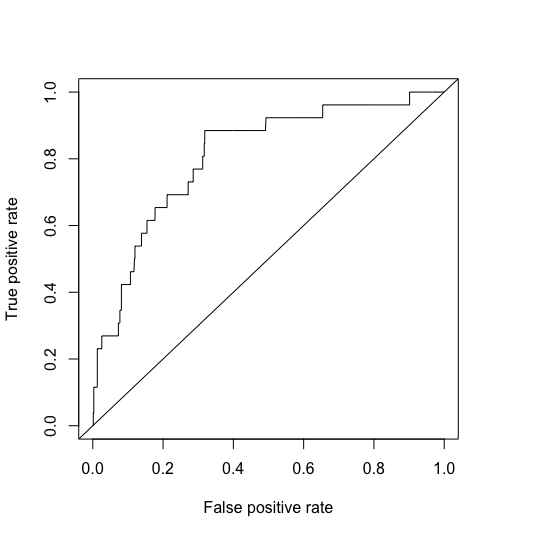
\includegraphics[width=9cm]{RFAUC.png}
  \label{fig:sub1}
  \caption{Random Forest Model Performance}
\end{figure}

\newpage

\section{Alternate Methods}
Due to the great class imbalance in our dataset, I experimented with synthetic re-sampling techniques to try and increase the sample size of failed drugs. The R package I conducted these experiments with was the SMOTE package. I attempted to over sample the failed drugs class to try and provide more instances of failed drugs to both the training set and test set. The best performance came when we doubled the size of the minority class, however even in this case the results were much worse then without any synthetic sampling. The best result achieved with any amount of oversampling present in the minority class was an area under the curve score of 0.6742, significantly worse than any of our original models. I believe the source of poor performance was a combination of only having 86 instances of the minority class to begin with and the significant number of features in the data (48 total features). Having so little data to start with was too large a barrier for SMOTE to overcome in order to provide high quality new instances. Therefore in the future if one wanted to make use of synthetic resampling, more instances of drugs that failed clinical trials due to toxicity would be required, however the entire purpose of oversampling this class is to prevent the need for further data collection so it is difficult to say whether synthetic sampling would ever be effective in this setting.  

\section{Discussion}
The performance of the gradient boosting version of PrOCTOR was very promising. The model outperformed the original PrOCTOR model in predicting drugs that failed clinical trials using a very comparable data set, both in terms of features and in number of samples. The difference in performance was not very large, further the new random forest model performed  well in testing as well which indicated that both types of learning algorithms are relatively successful at prediction using the dataset used in this project. A more extensive evaluation process may we required to safely conclude that gradient boosting methods are more effective than PrOCTOR's method (random forest) at predicting drug failures due to toxicity reasons. \\
Reflecting on the differences between my procedure and the methodology outlined in the PrOCTOR paper there are two significant points. The first is the discrepancy between the number of trees the gradient boosting model used (4402) and the number of trees the PrOCTOR model used (50). The number of trees for the gradient boosting model was calculated with the 'gbm.perf' command and thus is very reliable. In the PrOCTOR paper there is little to no discussion about how the number of trees was decided on or calculated, which leads to considering that possibly their random forest model may have not been trained properly or more simply they did not see it necessary to outline the exact tuning method utilized in their paper. The difference in number of trees used between the two models is just a point of curiosity. Another difference between methods is that of the training and test sets. The method for forming the training and tests sets in this project was discussed earlier. In the PrOCTOR paper, they discuss that a sub-sampling approach was used to help account for the class imbalance, where the FDA approved drugs were randomly sampled to be the same size of the failed drugs class, and that this process was repeated 30 times to reduce the odds of poor representatives being sampled. It seems that the PrOCTOR model then makes use of 30 independent models to compute the final prediction, by selecting the majority prediction for each drug from all 30 models. It is difficult to replicate this process because the paper fails to mention how they distinguish between the training and test sets of data. The other alternative is that PrOCTOR was trained and tested on the entire dataset which would have lead to artificially inflated performance. The lack of information in this area lead me to simply carry out my own distinct process, that I was confident with and would not artificially increase performance. There are a few other minor differences between methodologies. As mentioned before the dataset used for training the gradient boosting model appeared to be slightly different from the data used to train PrOCTOR originally.
Overall I am happy with the balance I found between replicating the PrOCTOR methodology exactly and conducting my own accurate and reliable testing. These results show that gradient boosting could potentially be a very powerful tool at predicting drug failure during clinical trials due to toxicity. Training another gradient boosting model with a reduced feature space showed that although in future collecting 48 features worth of data may be time consuming, it is crucial for extracting the optimal performance from the model. Finally conducting our own tests with a random forest model helped support our evidence that gradient boosting methods appear to have a minor advantage in terms of predictive performance in this setting over random forest models.

\newpage

\section{Sources}
\begin{enumerate}
  \item https://www.ncbi.nlm.nih.gov/pubmed/27642066
  \item http://citeseerx.ist.psu.edu/viewdoc/summary?doi=10.1.1.149.4944
  \item http://citeseerx.ist.psu.edu/viewdoc/summary?doi=10.1.1.60.3232
  \item https://github.com/kgayvert/PrOCTOR
  \item https://aact.ctti-clinicaltrials.org/
\end{enumerate}

\end{document}